\chapter{\IfLanguageName{dutch}{Stand van zaken}{State of the art}}%
\label{ch:stand-van-zaken}

% Tip: Begin elk hoofdstuk met een paragraaf inleiding die beschrijft hoe
% dit hoofdstuk past binnen het geheel van de bachelorproef. Geef in het
% bijzonder aan wat de link is met het vorige en volgende hoofdstuk.

% Pas na deze inleidende paragraaf komt de eerste sectiehoofding.

\section{Inleiding tot aanbevelingssystemen}
Aanbevelingssystemen zijn algoritmes en software tools met als doel om gepersonaliseerde aanbevelingen op basis van gelijkenis van items, gebruikersprofiel of andere kenmerken, te geven aan gebruikers \autocite{Patel2020, Patel2023}. De aanbevelingen worden gemaakt aan de hand van verschillende besluitvormingsprocessen, zoals welk nieuws hij leest, naar welke film hij kijkt of naar welke muziek hij luistert \autocite{Patel2017}. De kernfunctie van een aanbevelingssysteem is het voorspellen van de relevantie of voorkeur die een gebruiker aan een item zou toekennen, waarbij de enorme hoveelheid informatie gefilterd wordt en gebruikers enkel keuzes krijgen voorgeschoteld die op hun interesses zijn afgestemd \autocite{Fkih2022}. Anders gezegd kunnen aanbevelingssystemen gezien worden als functies die informatie over de voorkeuren van een gebruiker (bijv. over films) als invoer nemen en een voorspelling doen over de beoordeling die een gebruiker zou geven aan andere gewenste items (bijv. nieuwe beschikbare films) en het uitvoer zijn aanbevelingen van deze items \autocite{Milano2020}. Aanbevelingen kunnen gaan over een breed scala aan items, waaronder producten in e-commerce, films, muziek, nieuwsartikelen en contacten op sociale media.
\subsection{Toepassingen van aanbevelingssystemen}
De toepassingen van aanbevelingssystemen zijn uitgebreid en doordringen talloze domeinen. Een van de meeste bekende toepassing is in e-commerce, waar producten aanbevelen aan klanten op basis van hun aankoopgeschiedenis en surfgedrag, zoals de Amazon \"item-to-item \ac{cf}\" algoritme \autocite{Patel2023, Patel2020}.
In de entertaintment industrie bij het aanbevelen van films op Netflix, IMDB of MovieLens en muziek \autocite{Patel2020, Roy2022}. Op sociale media platformen zoals Facebook en Twitter worden aanbevelingen gedaan voor nieuwe personen en pagina's te ontdekken \autocite{Patel2023}. Zelfs de advertenties op deze platformen zijn vaak afgestemd op de intresses van de gebruiker \autocite{Patel2020}.
In het onderzoek \textcite{Agapito2016} wordt DIETOS (DIET Organizer System) geïntroduceerd, een webgebaseerd aanbevelingssysteem dat gepersonaliseerd voedingsadvies biedt op basis van een gezondheidsprofiel van de gebruiker. Dit profiel wordt opgebouwd via dynamische vragenlijsten die zijn ontwikkeld en gevalideerd door medische professionals. Het systeem richt zich specifiek op het aanbevelen van geschikte voedingsmiddelen voor personen met chronische aandoeningen zoals diabetes, hypertensie en chronische nierziekten. Toeristen kunnen ook geholpen worden bij het plannen van hun reis door aanbevelingen te geven over bezienswaardigheden, restaurants en hotels \autocite{Roy2022, Patel2023}.
\subsection{Wat maakt ze nuttig?}
Tegenwoordig wordt overweldigende data geproduceerd waardoor gebruikers makkelijk overbeslast kunnen worden met informatie en keuzes. Een gebruiker zou zelf door de data moeten filteren om het gewenst item te vinden. Aanbevelingssystemen bieden een oplossing voor dit probleem door data te analyseren en te filteren om nuttige informatie te extraheren \autocite{Fkih2022}. Ze zijn in staat om gebruikersvoorkeuren en gedrag te voorspellen waardoor ze kunnen inspelen op de behoeften van de gebruiker \autocite{Mazeh2020}. Ze verbeteren de besluitvorming van gebruikers door relevante opties voor te stellen, zoals wat te kopen, te lezen of te bekijken, en moedigen hen aan om actie te ondernemen \autocite{Mazeh2020}. Daarnaast spelen aanbevelingssystemen een belangrijke rol in het creëren van bedrijfswaarde, doordat ze bijdragen aan verkoop en omzet door producten aan te bevelen die klanten waarschijnlijk zullen kopen \autocite{Wang2018, Patel2023}. \autocite{MacKenzie2013} toont aan dat 35\% van de aankopen op Amazon en 75\% van wat gebruikers op Netflix bekijken, te danken is aan gepersonaliseerde aanbevelingen. Huidige cijfers zijn waarschijnlijk nog hoger.
\subsection{Soorten aanbevelingssystemen}
\begin{figure}
  \centering
  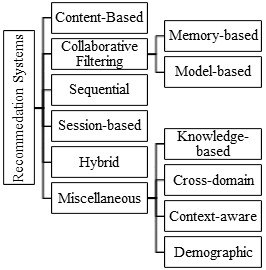
\includegraphics[width=0.4\textwidth]{taxonomie-rs-patel2023.jpg}
  \caption[Taxonomie van aanbevelingssystemen]{\label{fig:TaxonomieRS} Taxonomie van aanbevelingssystemen \autocite{Patel2023}}
\end{figure}

\section{\ac{cf} gebaseerde aanbevelingssystemen}
\section{Toepassing \ac{fl} techniek}
\section{\ac{dp} framework}
\section{Evalueren van aanbevelingssystemen}

Dit hoofdstuk bevat je literatuurstudie. De inhoud gaat verder op de inleiding, maar zal het onderwerp van de bachelorproef *diepgaand* uitspitten. De bedoeling is dat de lezer na lezing van dit hoofdstuk helemaal op de hoogte is van de huidige stand van zaken (state-of-the-art) in het onderzoeksdomein. Iemand die niet vertrouwd is met het onderwerp, weet nu voldoende om de rest van het verhaal te kunnen volgen, zonder dat die er nog andere informatie moet over opzoeken \autocite{Pollefliet2011}.

Je verwijst bij elke bewering die je doet, vakterm die je introduceert, enz.\ naar je bronnen. In \LaTeX{} kan dat met het commando \texttt{$\backslash${textcite\{\}}} of \texttt{$\backslash${autocite\{\}}}. Als argument van het commando geef je de ``sleutel'' van een ``record'' in een bibliografische databank in het Bib\LaTeX{}-formaat (een tekstbestand). Als je expliciet naar de auteur verwijst in de zin (narratieve referentie), gebruik je \texttt{$\backslash${}textcite\{\}}. Soms is de auteursnaam niet expliciet een onderdeel van de zin, dan gebruik je \texttt{$\backslash${}autocite\{\}} (referentie tussen haakjes). Dit gebruik je bv.~bij een citaat, of om in het bijschrift van een overgenomen afbeelding, broncode, tabel, enz. te verwijzen naar de bron. In de volgende paragraaf een voorbeeld van elk.

\textcite{Knuth1998} schreef een van de standaardwerken over sorteer- en zoekalgoritmen. Experten zijn het erover eens dat cloud computing een interessante opportuniteit vormen, zowel voor gebruikers als voor dienstverleners op vlak van informatietechnologie~\autocite{Creeger2009}.

Let er ook op: het \texttt{cite}-commando voor de punt, dus binnen de zin. Je verwijst meteen naar een bron in de eerste zin die erop gebaseerd is, dus niet pas op het einde van een paragraaf.

\begin{figure}
  \centering
  \includegraphics[width=0.8\textwidth]{grail.jpg}
  \caption[Voorbeeld figuur.]{\label{fig:grail}Voorbeeld van invoegen van een figuur. Zorg altijd voor een uitgebreid bijschrift dat de figuur volledig beschrijft zonder in de tekst te moeten gaan zoeken. Vergeet ook je bronvermelding niet!}
\end{figure}

\begin{listing}
  \begin{minted}{python}
    import pandas as pd
    import seaborn as sns

    penguins = sns.load_dataset('penguins')
    sns.relplot(data=penguins, x="flipper_length_mm", y="bill_length_mm", hue="species")
  \end{minted}
  \caption[Voorbeeld codefragment]{Voorbeeld van het invoegen van een codefragment.}
\end{listing}

\lipsum[7-20]

\begin{table}
  \centering
  \begin{tabular}{lcr}
    \toprule
    \textbf{Kolom 1} & \textbf{Kolom 2} & \textbf{Kolom 3} \\
    $\alpha$         & $\beta$          & $\gamma$         \\
    \midrule
    A                & 10.230           & a                \\
    B                & 45.678           & b                \\
    C                & 99.987           & c                \\
    \bottomrule
  \end{tabular}
  \caption[Voorbeeld tabel]{\label{tab:example}Voorbeeld van een tabel.}
\end{table}

